% Created 2021-08-31 Tue 14:00
% Intended LaTeX compiler: pdflatex
\documentclass[11pt]{article}
\usepackage[utf8]{inputenc}
\usepackage[T1]{fontenc}
\usepackage{graphicx}
\usepackage{grffile}
\usepackage{longtable}
\usepackage{wrapfig}
\usepackage{rotating}
\usepackage[normalem]{ulem}
\usepackage{amsmath}
\usepackage{textcomp}
\usepackage{amssymb}
\usepackage{capt-of}
\usepackage{hyperref}
\author{David Lewis}
\date{\today}
\title{}
\hypersetup{
 pdfauthor={David Lewis},
 pdftitle={},
 pdfkeywords={},
 pdfsubject={},
 pdfcreator={Emacs 28.0.50 (Org mode 9.5)}, 
 pdflang={English}}
\begin{document}

\tableofcontents

\section{Abstract}
\label{sec:org673c52e}
\section{Introduction}
\label{sec:orga234600}
\section{Methods}
\label{sec:org461de2b}
\subsection{Transcriptomic Workflow Overview}
\label{sec:orgd2cd0a0}
\begin{center}
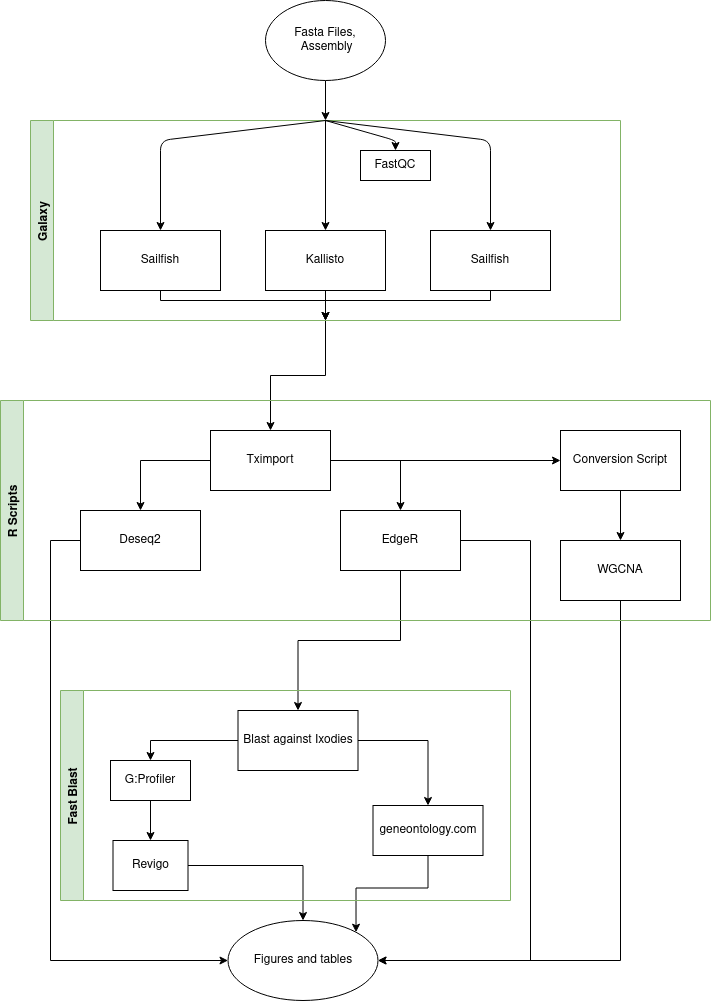
\includegraphics[width=.9\linewidth]{Workflow.png}
\end{center}
\subsubsection{Quantification}
\label{sec:orgf0e41a5}
The Raw high-throughput RNA-sequencing data from each trial were saved as individual FASTQ files.
The FASTQ files were uploaded to the Galaxy platform (\texttt{usegalaxy.org} ) where the quantifiaction occured.
First, Galaxy's 'FastQC' tool was used to determine the quality of the raw data and to mitigate the effects of amplification bias \texttt{insert settings here}). The Kmer test within 'FastQC' was enabled and set at a length of 7bp.
Following this initial quality-check, the raw files were trimmed with 'Trimmomatic' using its default settings (\texttt{description}).
FastQC was run on the trimmed files to confirm its quality.

After the data was trimmed, transcript abundance quantifiaction was performed by the Galaxy's 'Sailfish quant' tool using the default settings (\texttt{description}).
\subsection{Differential expression analysis}
\label{sec:org71dd47e}
DESeq2(\texttt{Reference}) and EdgeR(\texttt{Reference}) were used to test for differential expression between the legs, body, and pesticide treatment (Deet and Perm). The transcript-level counts were quantified using the TPM (transcripts per million) generated from the 'Sailfish quant' tool. The differentially expressed genes were estimated using an adjusted p value cutoff of less than 0.05 for multiple testing using a false discover rate FDR)   (Benjamini   and   Hochberg,  1995),   and   a   log 2 -fold   change   ≥   |2|.
The differential analysis becomes more reliable when the results of the similar tools are compared.
\subsection{WGCNA}
\label{sec:org8b88d21}
\subsection{GO analysis}
\label{sec:org1492adf}
\subsubsection{Blast}
\label{sec:org67be582}
The significantly differentially expressed contigs were searched (BLASTx) against the NCBI \emph{Ixodies scapularis} SwissProt protein database with an expectation value (e-value) of 0.001.
The highest scoring blast hits were assigned a gene ID for each contig.
Fore each search, a positive BLAST hit was functionally profiled using g:Profiler and the PANTHER Classification System.
\subsubsection{GProfiler}
\label{sec:org7926636}
Functional profiling of overrepresented gene sets were statistically listed with enriched terms in gProfiler.
g:GOSt was the g-profiler tool used for functional enrichment analysis.
The GProfiler output is sent to Revigo.
\subsubsection{Revigo}
\label{sec:org70b0d3f}
The R script output of REVIGO (Rudjer Boskovic Institute) generates tree-maps of the genes. These maps show the function of the enriched genes.
\subsubsection{Geneontolyg.org}
\label{sec:orgd728dbd}
The ouptut of blast is sent to Geneontology.org (not sure if this section is needed (didn't use the data at all))
\section{Results}
\label{sec:orgf8494aa}
\subsection{Figure 1: methods comparison between EdgeR and Deseq2}
\label{sec:org1bf6993}
This figure compares the differential expression data from both EdgeR and Deseq2. The P value is small, indicating that EdgeR and Deseq2 have similar results.

\begin{center}
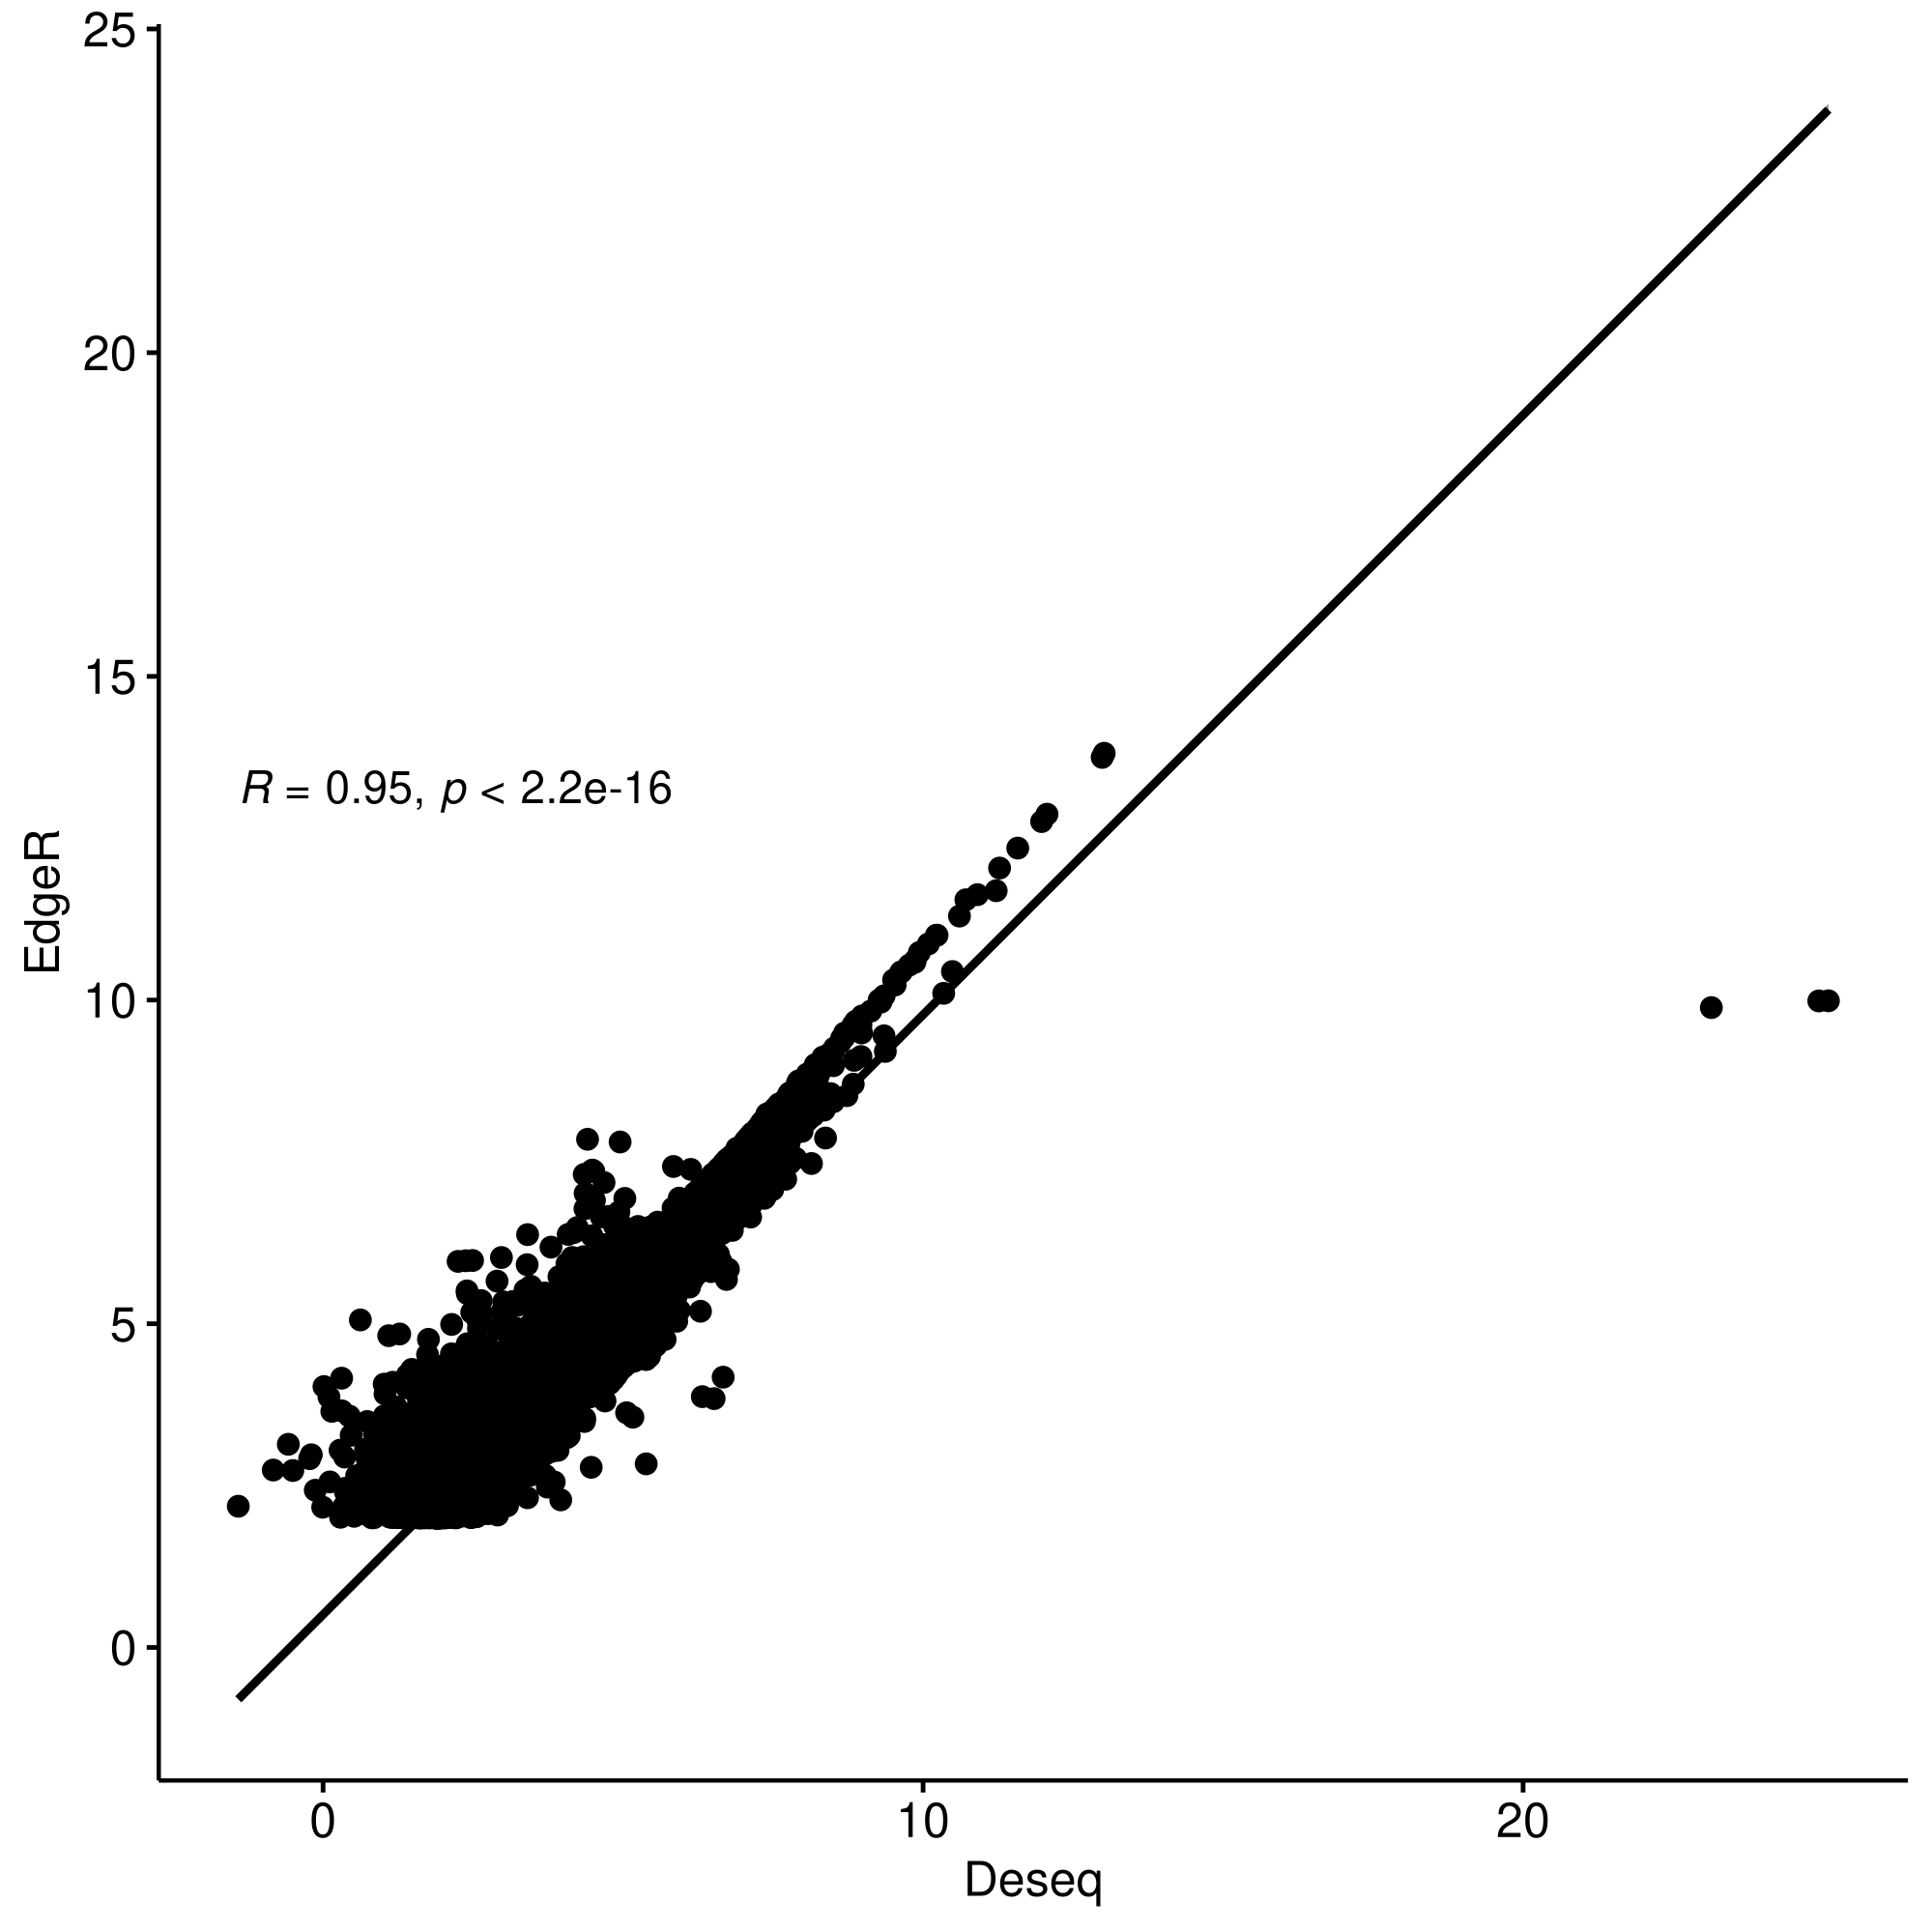
\includegraphics[width=0.6\textwidth]{figure1/pearson.png}
\captionof{figure}{The quantification files were run through both EdgeR and Deseq2. Each axis plots the expression values as given by its respective title.}
\end{center}
\subsection{Figure 2: Perm and Deet repellency and survival}
\label{sec:org60543b7}
\subsection{Figure 3: Leg vs Body general (control)}
\label{sec:orgce86978}
\begin{center}
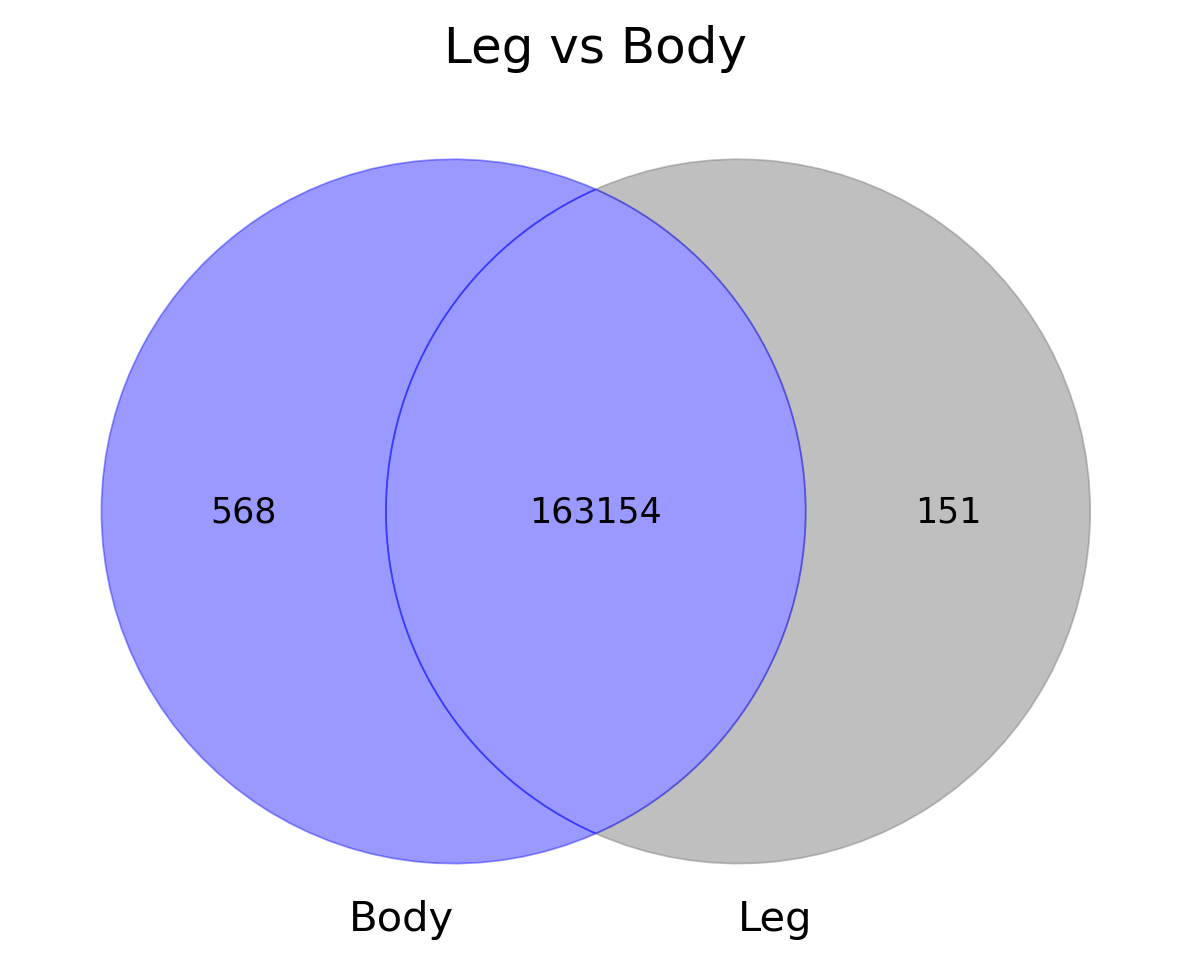
\includegraphics[width=0.6\textwidth]{figure3/Deseq-BodyvsLeg.png}
\captionof{figure}{Comparison of up-regulated genes in the body and leg compared to the total number of genes from the sample.}
\end{center}
\subsubsection{{\bfseries\sffamily TODO} supplemental tables}
\label{sec:org18f899d}
\subsection{Figure 4: Leg vs Body Specifics overlap with Ixodies}
\label{sec:org001c7de}
Refer to paper in google drive. Discussion.
\subsection{Figure 5:Response to DEET In Leg and Body}
\label{sec:org5268e66}
\subsubsection{Body}
\label{sec:orgce98a64}
\begin{center}
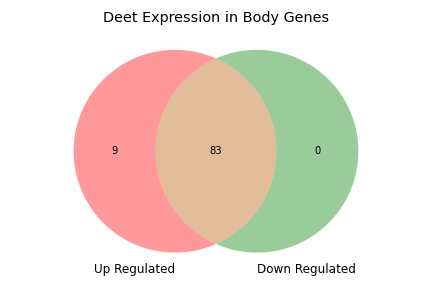
\includegraphics[width=0.6\textwidth]{figure5/DeetBodyDeseq.png}
\captionof{figure}{Differentially expressed genes with respect to the body are further compared based on differential expression with respect to the Deet comparison.}
\end{center}
\subsubsection{Leg}
\label{sec:orgce0e1d8}
\begin{center}
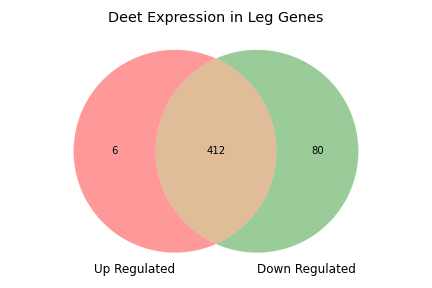
\includegraphics[width=0.6\textwidth]{figure5/DeetLegDeseq.png}
\captionof{figure}{Differentially expressed genes with respect to the leg are further compared based on differential expression with respect to the Deet comparison.}
\end{center}
\subsubsection{{\bfseries\sffamily TODO} supplemental tables}
\label{sec:org37ba1d8}
\subsection{Figure 6: Response to PERM in Leg and Body}
\label{sec:orgac833e6}
\subsubsection{Body}
\label{sec:orga86a084}
\begin{center}
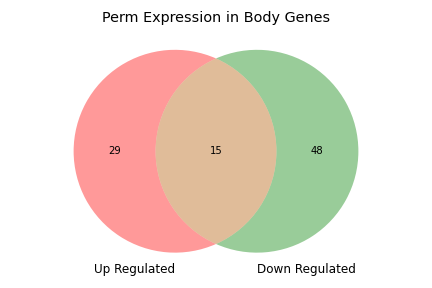
\includegraphics[width=0.6\textwidth]{figure6/PermBodyDeseq.png}
\captionof{figure}{Differentially expressed genes with respect to the body are further compared based on differential expression with respect to the Perm comparison.}
\end{center}
\subsubsection{Leg}
\label{sec:orgd785b30}
\begin{center}
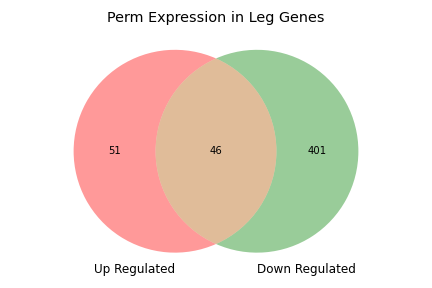
\includegraphics[width=0.6\textwidth]{figure6/PermLegDeseq.png}
\captionof{figure}{Differentially expressed genes with respect to the leg are further compared based on differential expression with respect to the Perm comparison.}
\end{center}
\subsubsection{{\bfseries\sffamily TODO} supplemental tables}
\label{sec:org75379a0}
\subsection{Figure 7: WGCNA}
\label{sec:org012262b}
\subsection{Figure 8: Overlap Between the response, body and leg}
\label{sec:org4aa5cb9}
Don't think we need it now.
\subsection{Figure 9: Time Course Legs}
\label{sec:orgac3c73d}
\subsubsection{DEET}
\label{sec:orgfd6a939}
\begin{center}
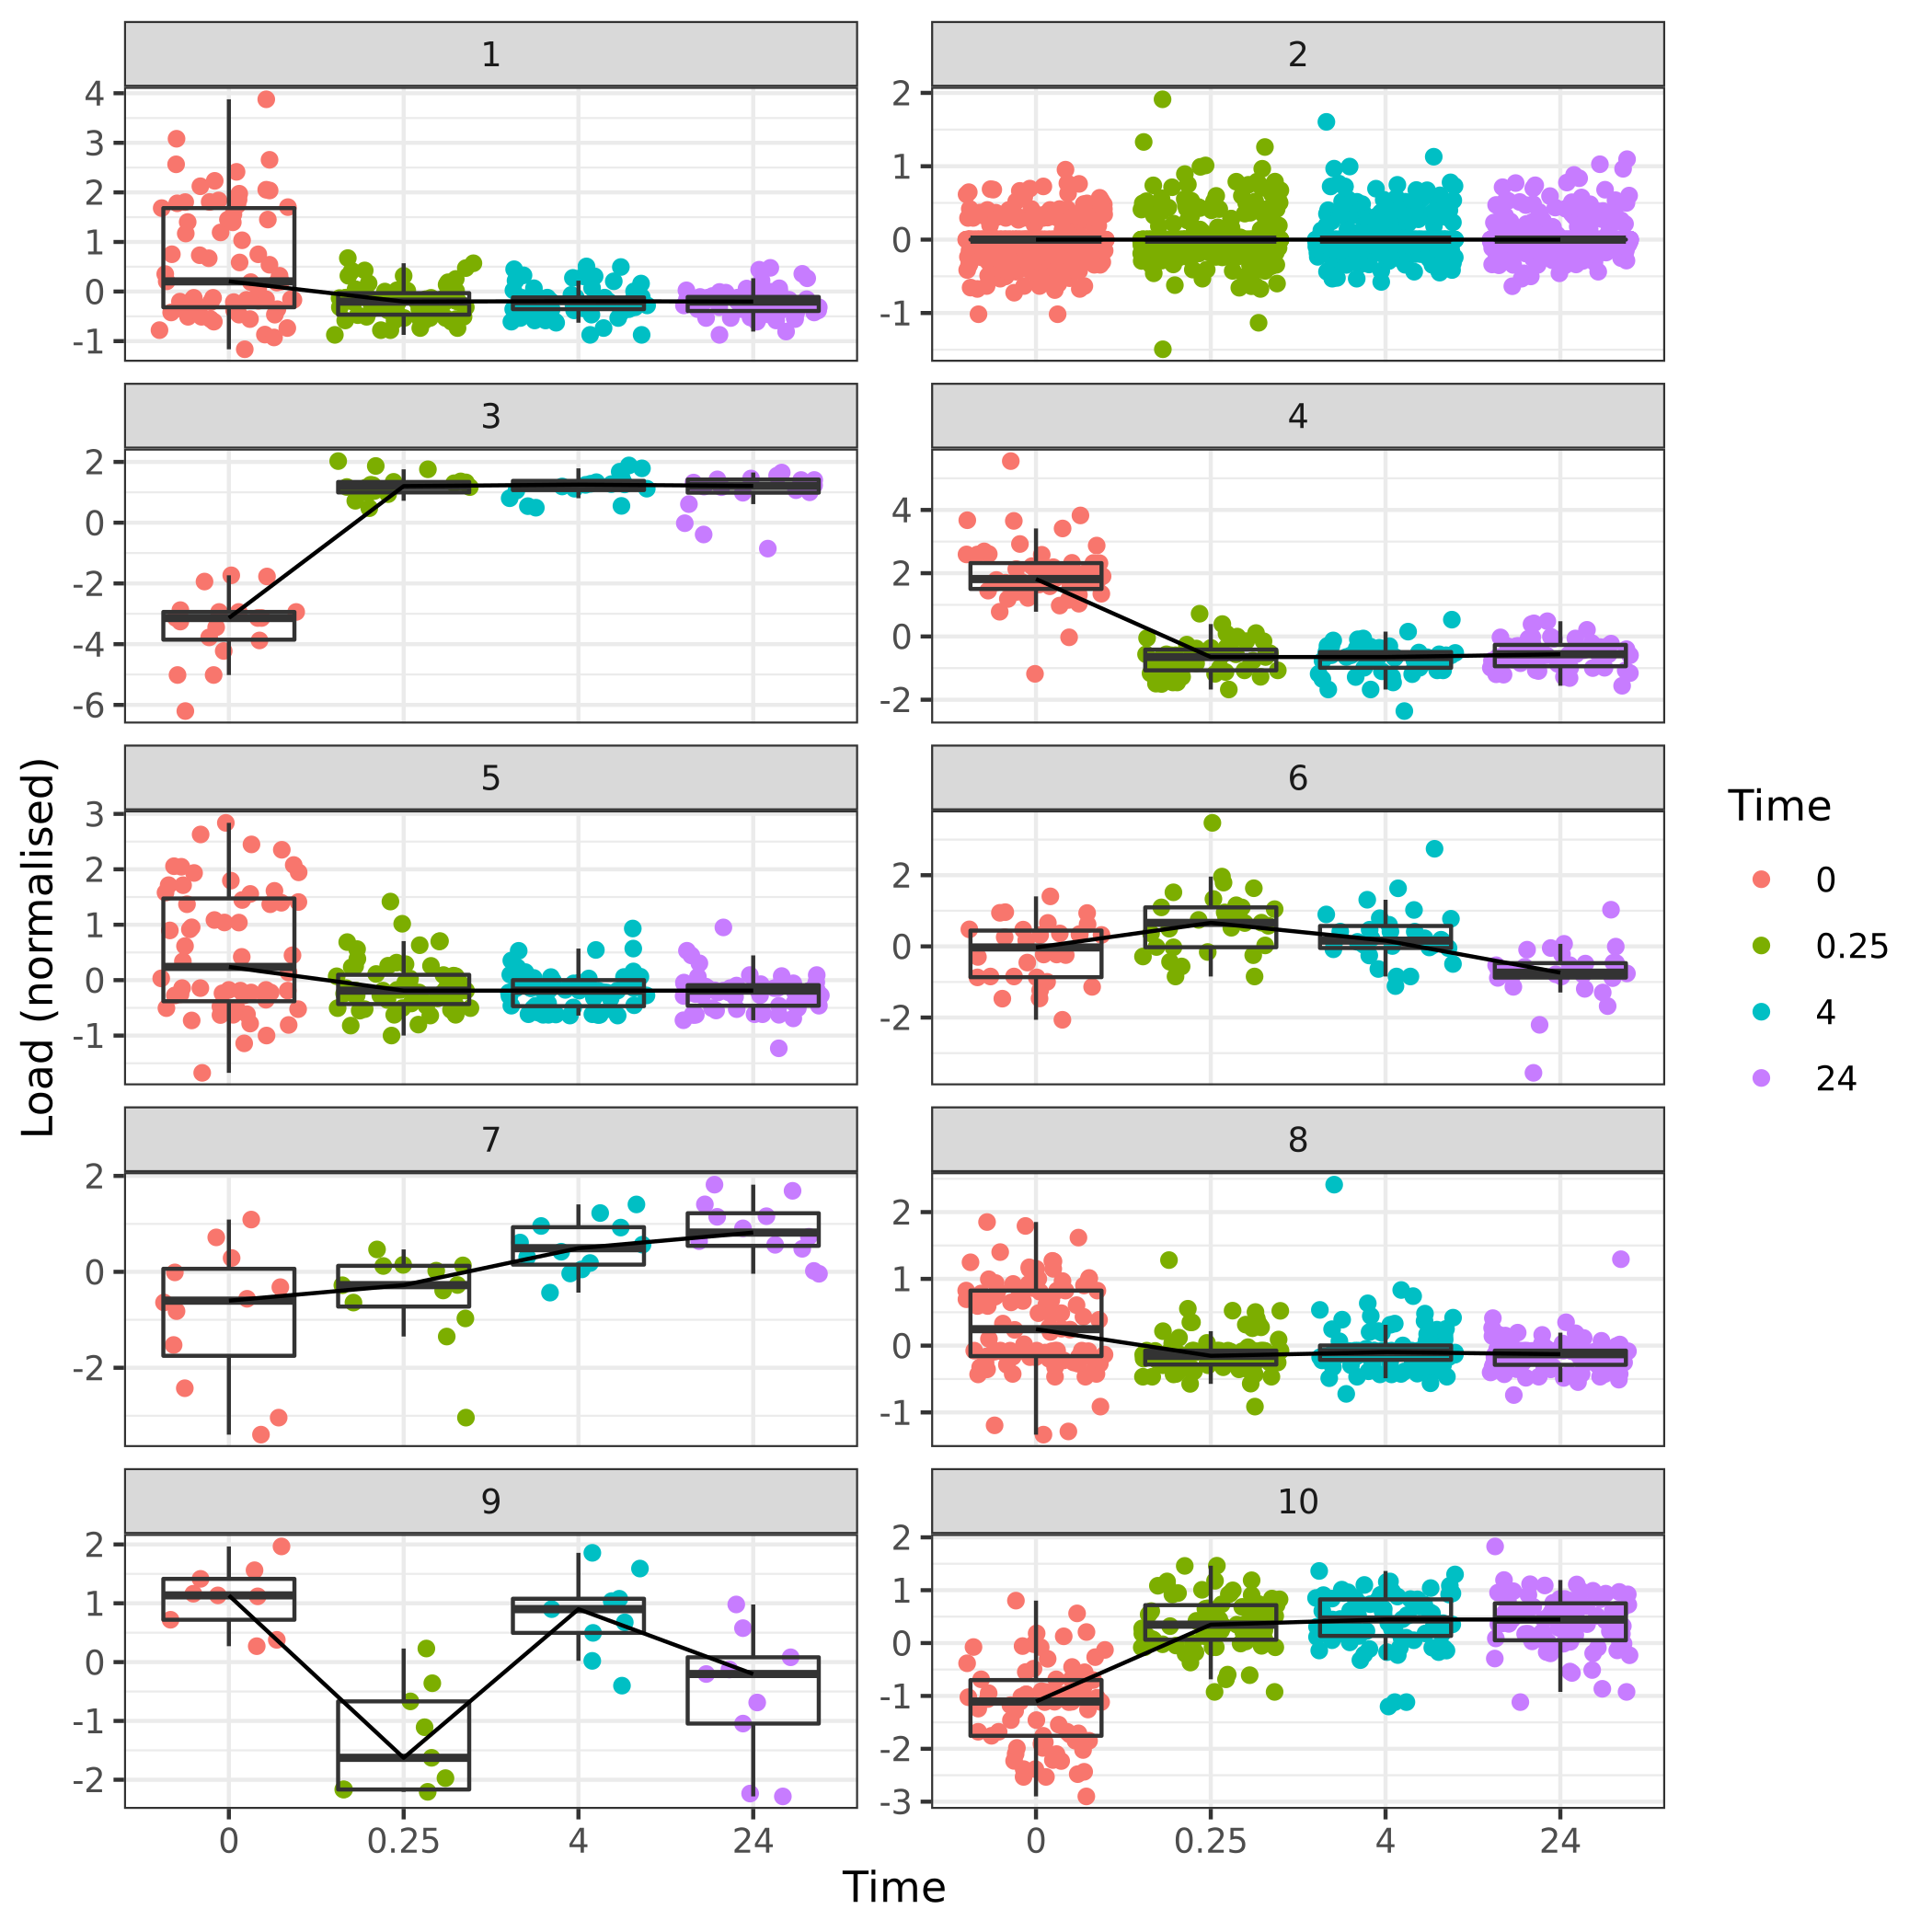
\includegraphics[width=0.6\textwidth]{figure9/DEET/Legbox.png}
\end{center}
\begin{enumerate}
\item Supplemental Tables
\label{sec:org3d6e145}
\url{figure9/DEET/Legbox}
\end{enumerate}
\subsubsection{PERM}
\label{sec:orgf75c4fd}
\begin{center}
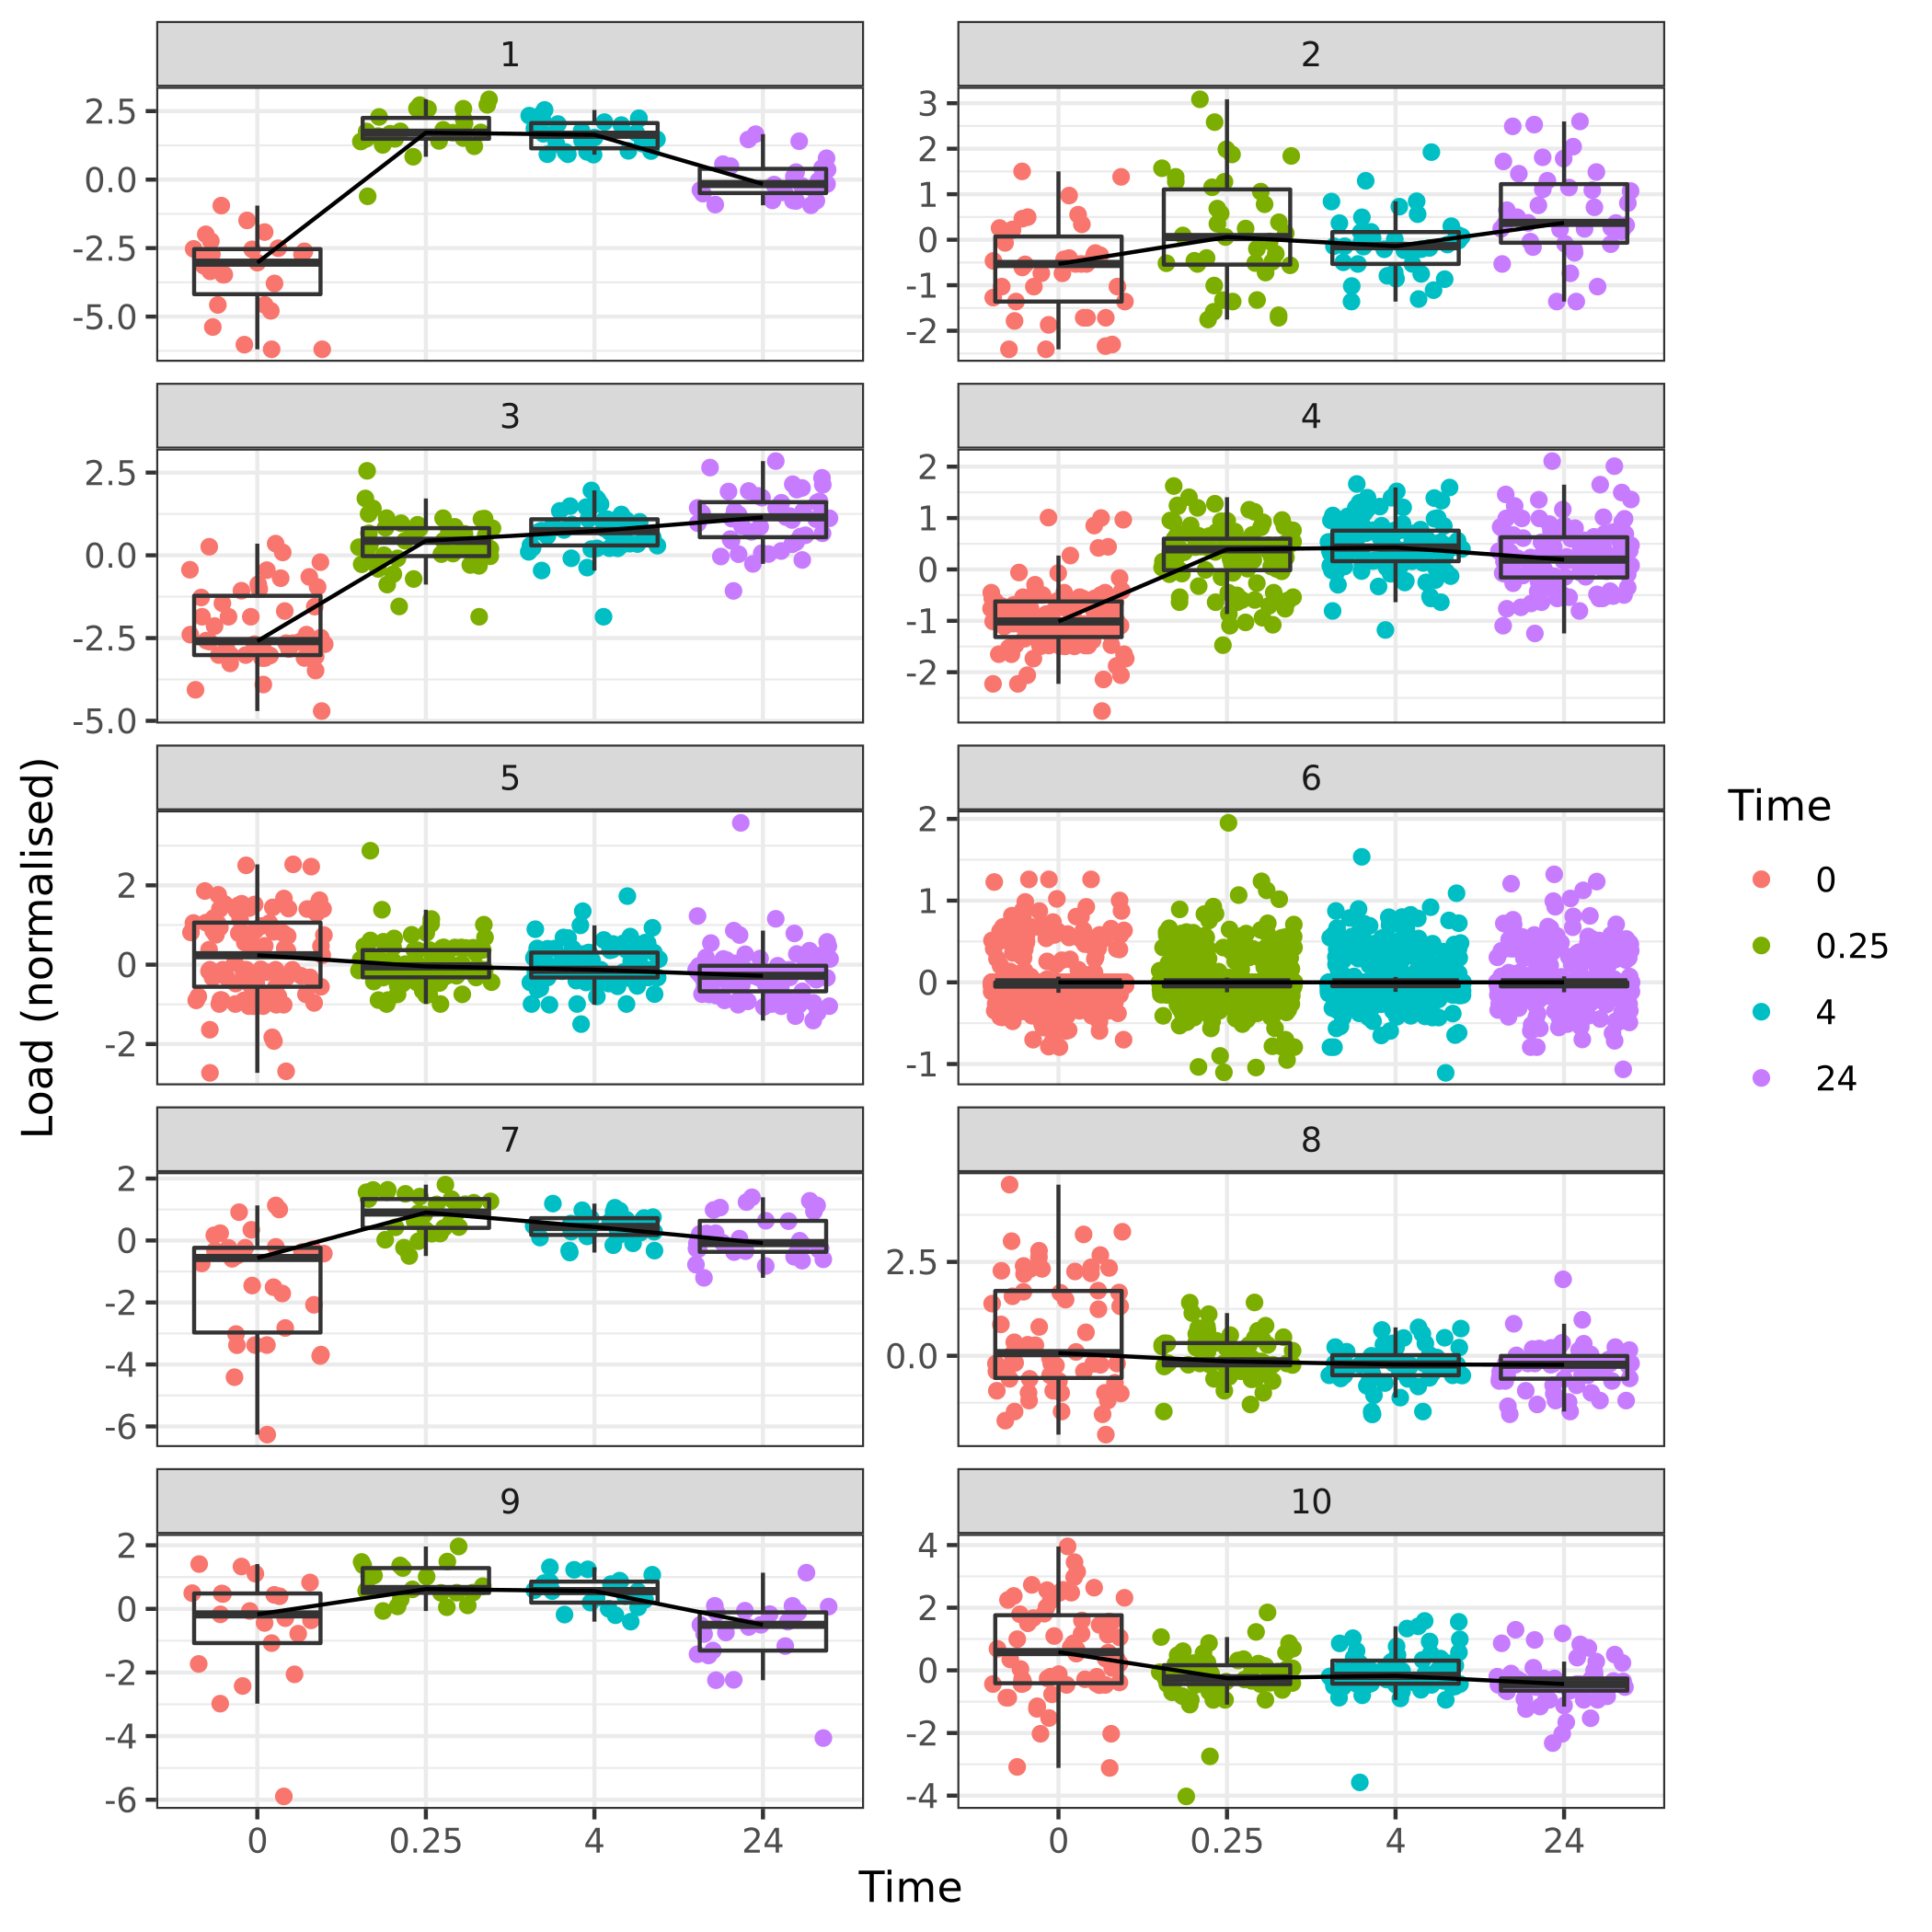
\includegraphics[width=0.6\textwidth]{figure9/PERM/Legbox.png}
\end{center}
\begin{enumerate}
\item Supplemental Tables
\label{sec:org740262e}
\url{figure9/PERM/Legbox}
\end{enumerate}
\subsection{Figure 10: Time Course Body}
\label{sec:org42e7e0f}
\subsubsection{DEET}
\label{sec:orge600387}
\begin{center}
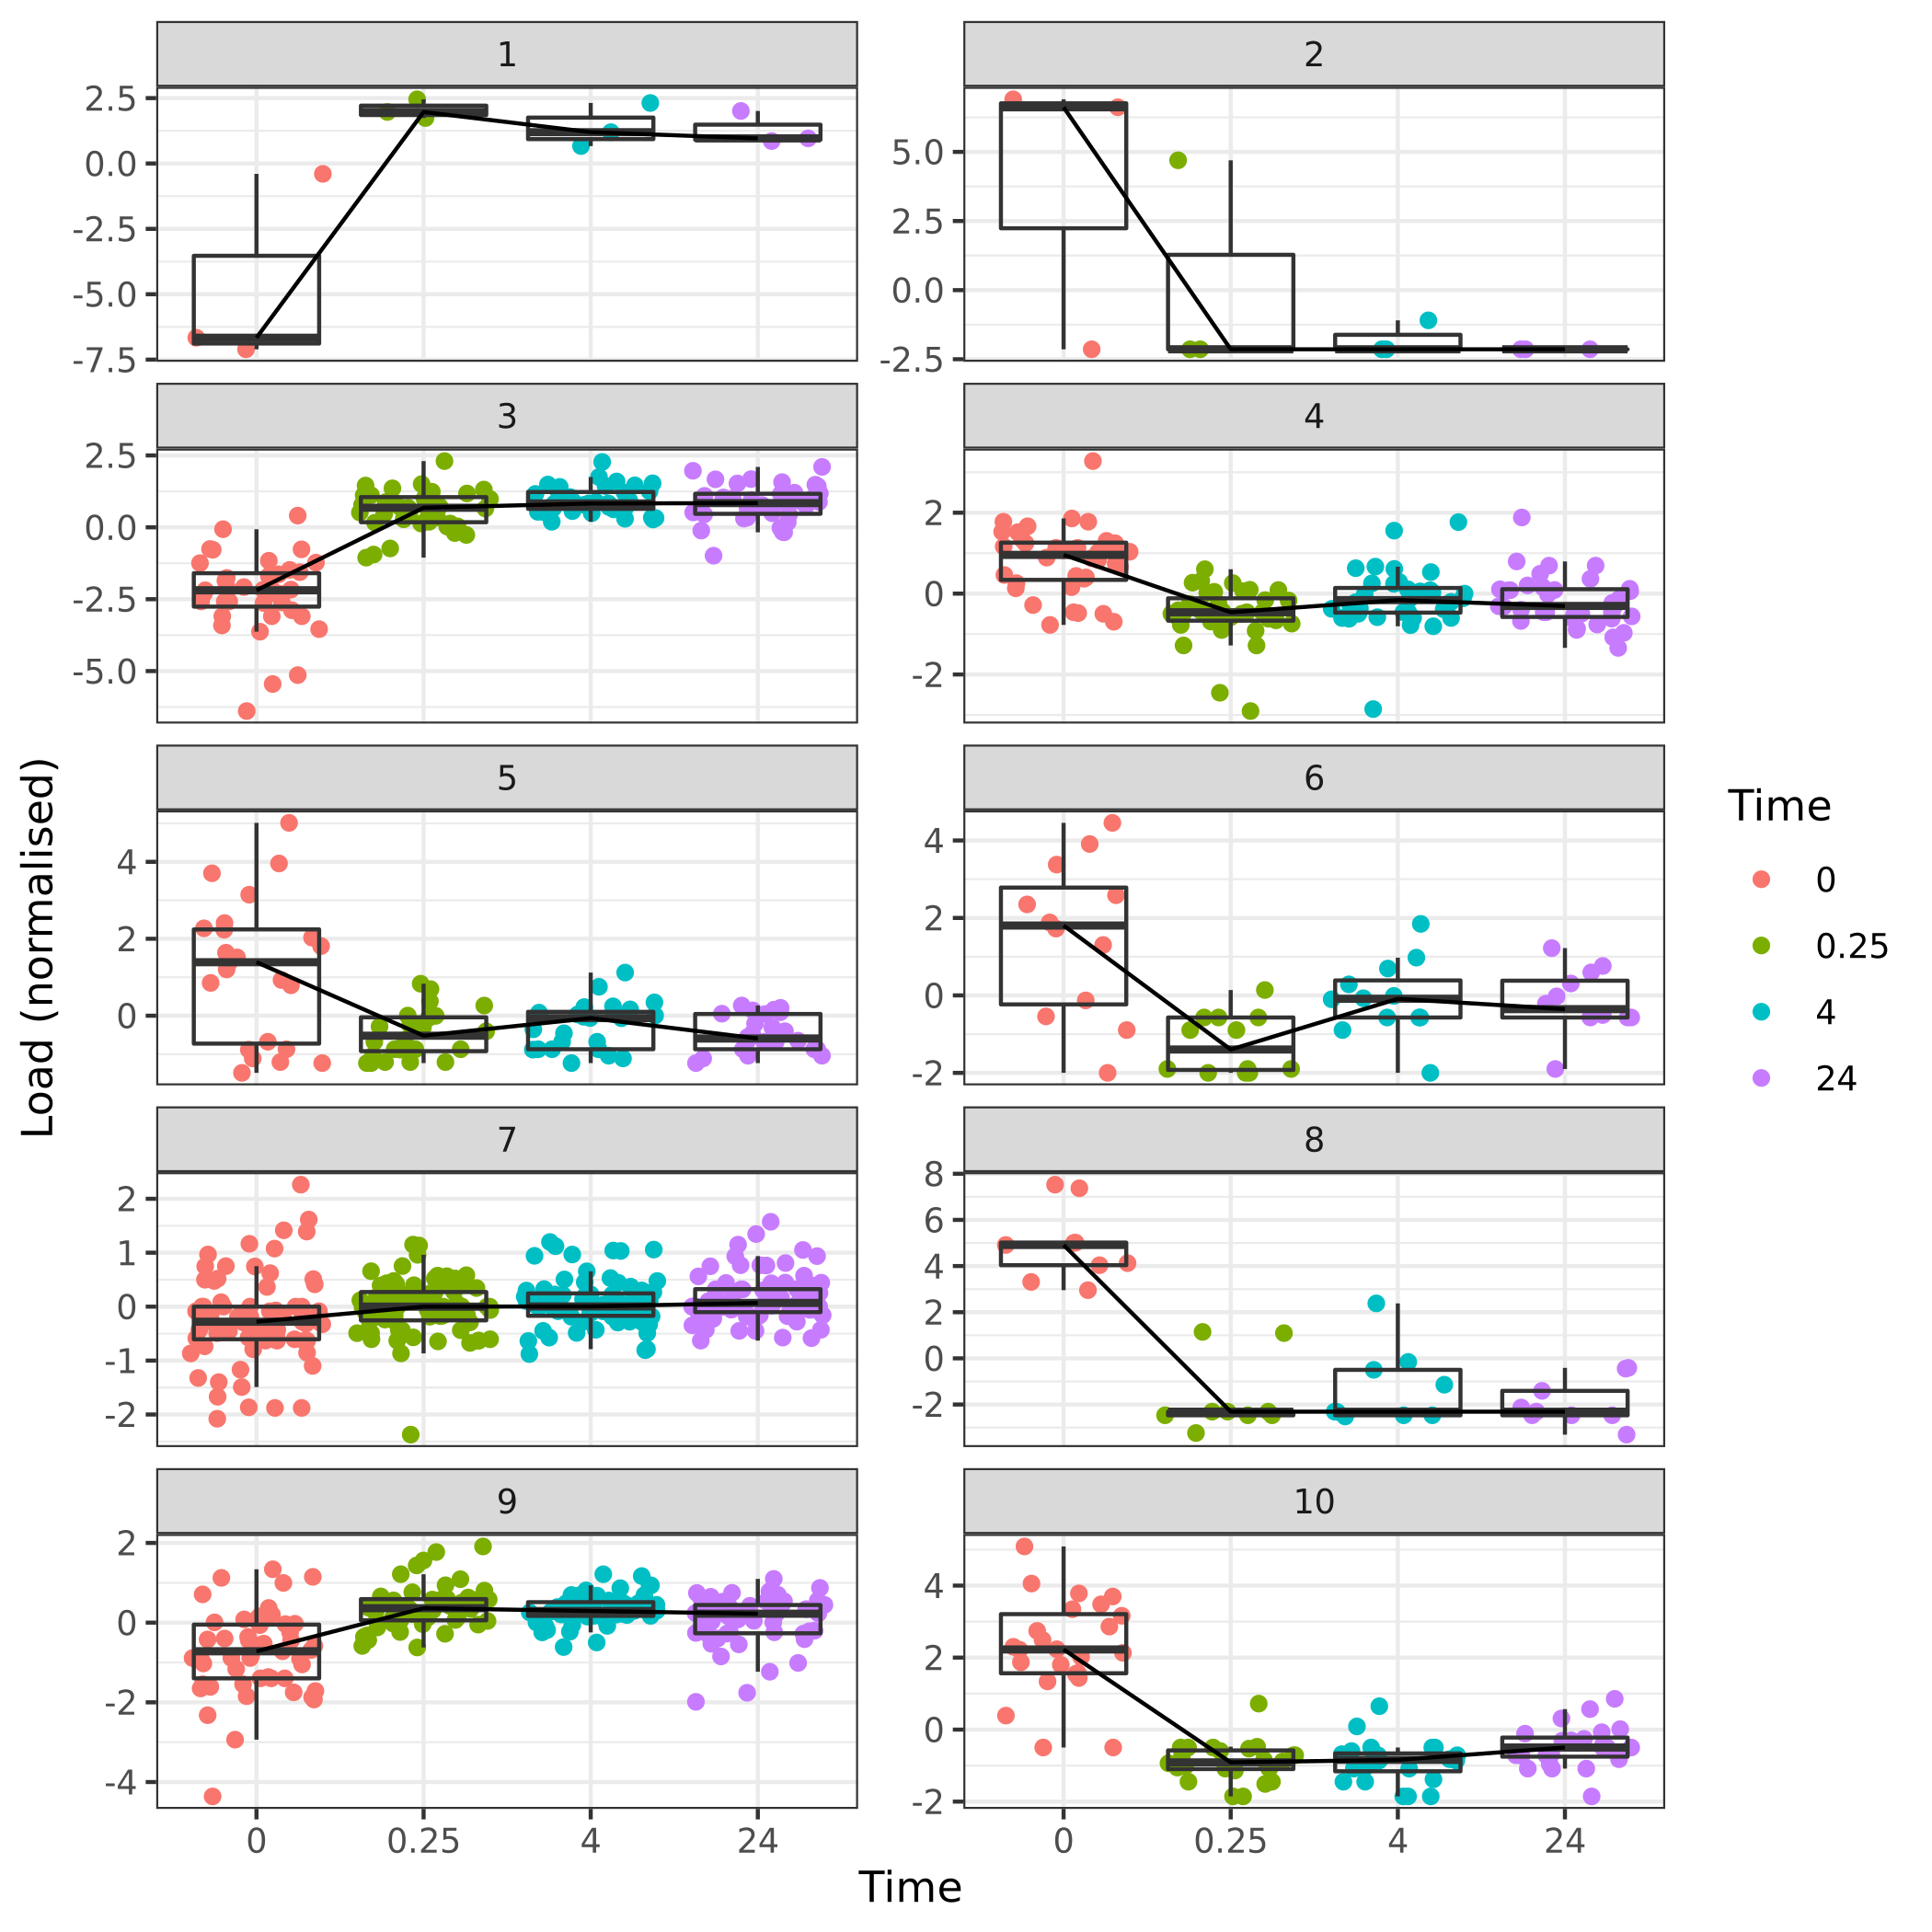
\includegraphics[width=0.6\textwidth]{figure10/DEET/Bodybox.png}
\captionof{figure}{K-mean clusters of differential expression data}
\end{center}
\begin{enumerate}
\item Supplemental Tables
\label{sec:orgcde0dbf}
\url{figure10/DEET/Bodybox/}
\end{enumerate}
\subsubsection{PERM}
\label{sec:org87a18f0}
\begin{center}
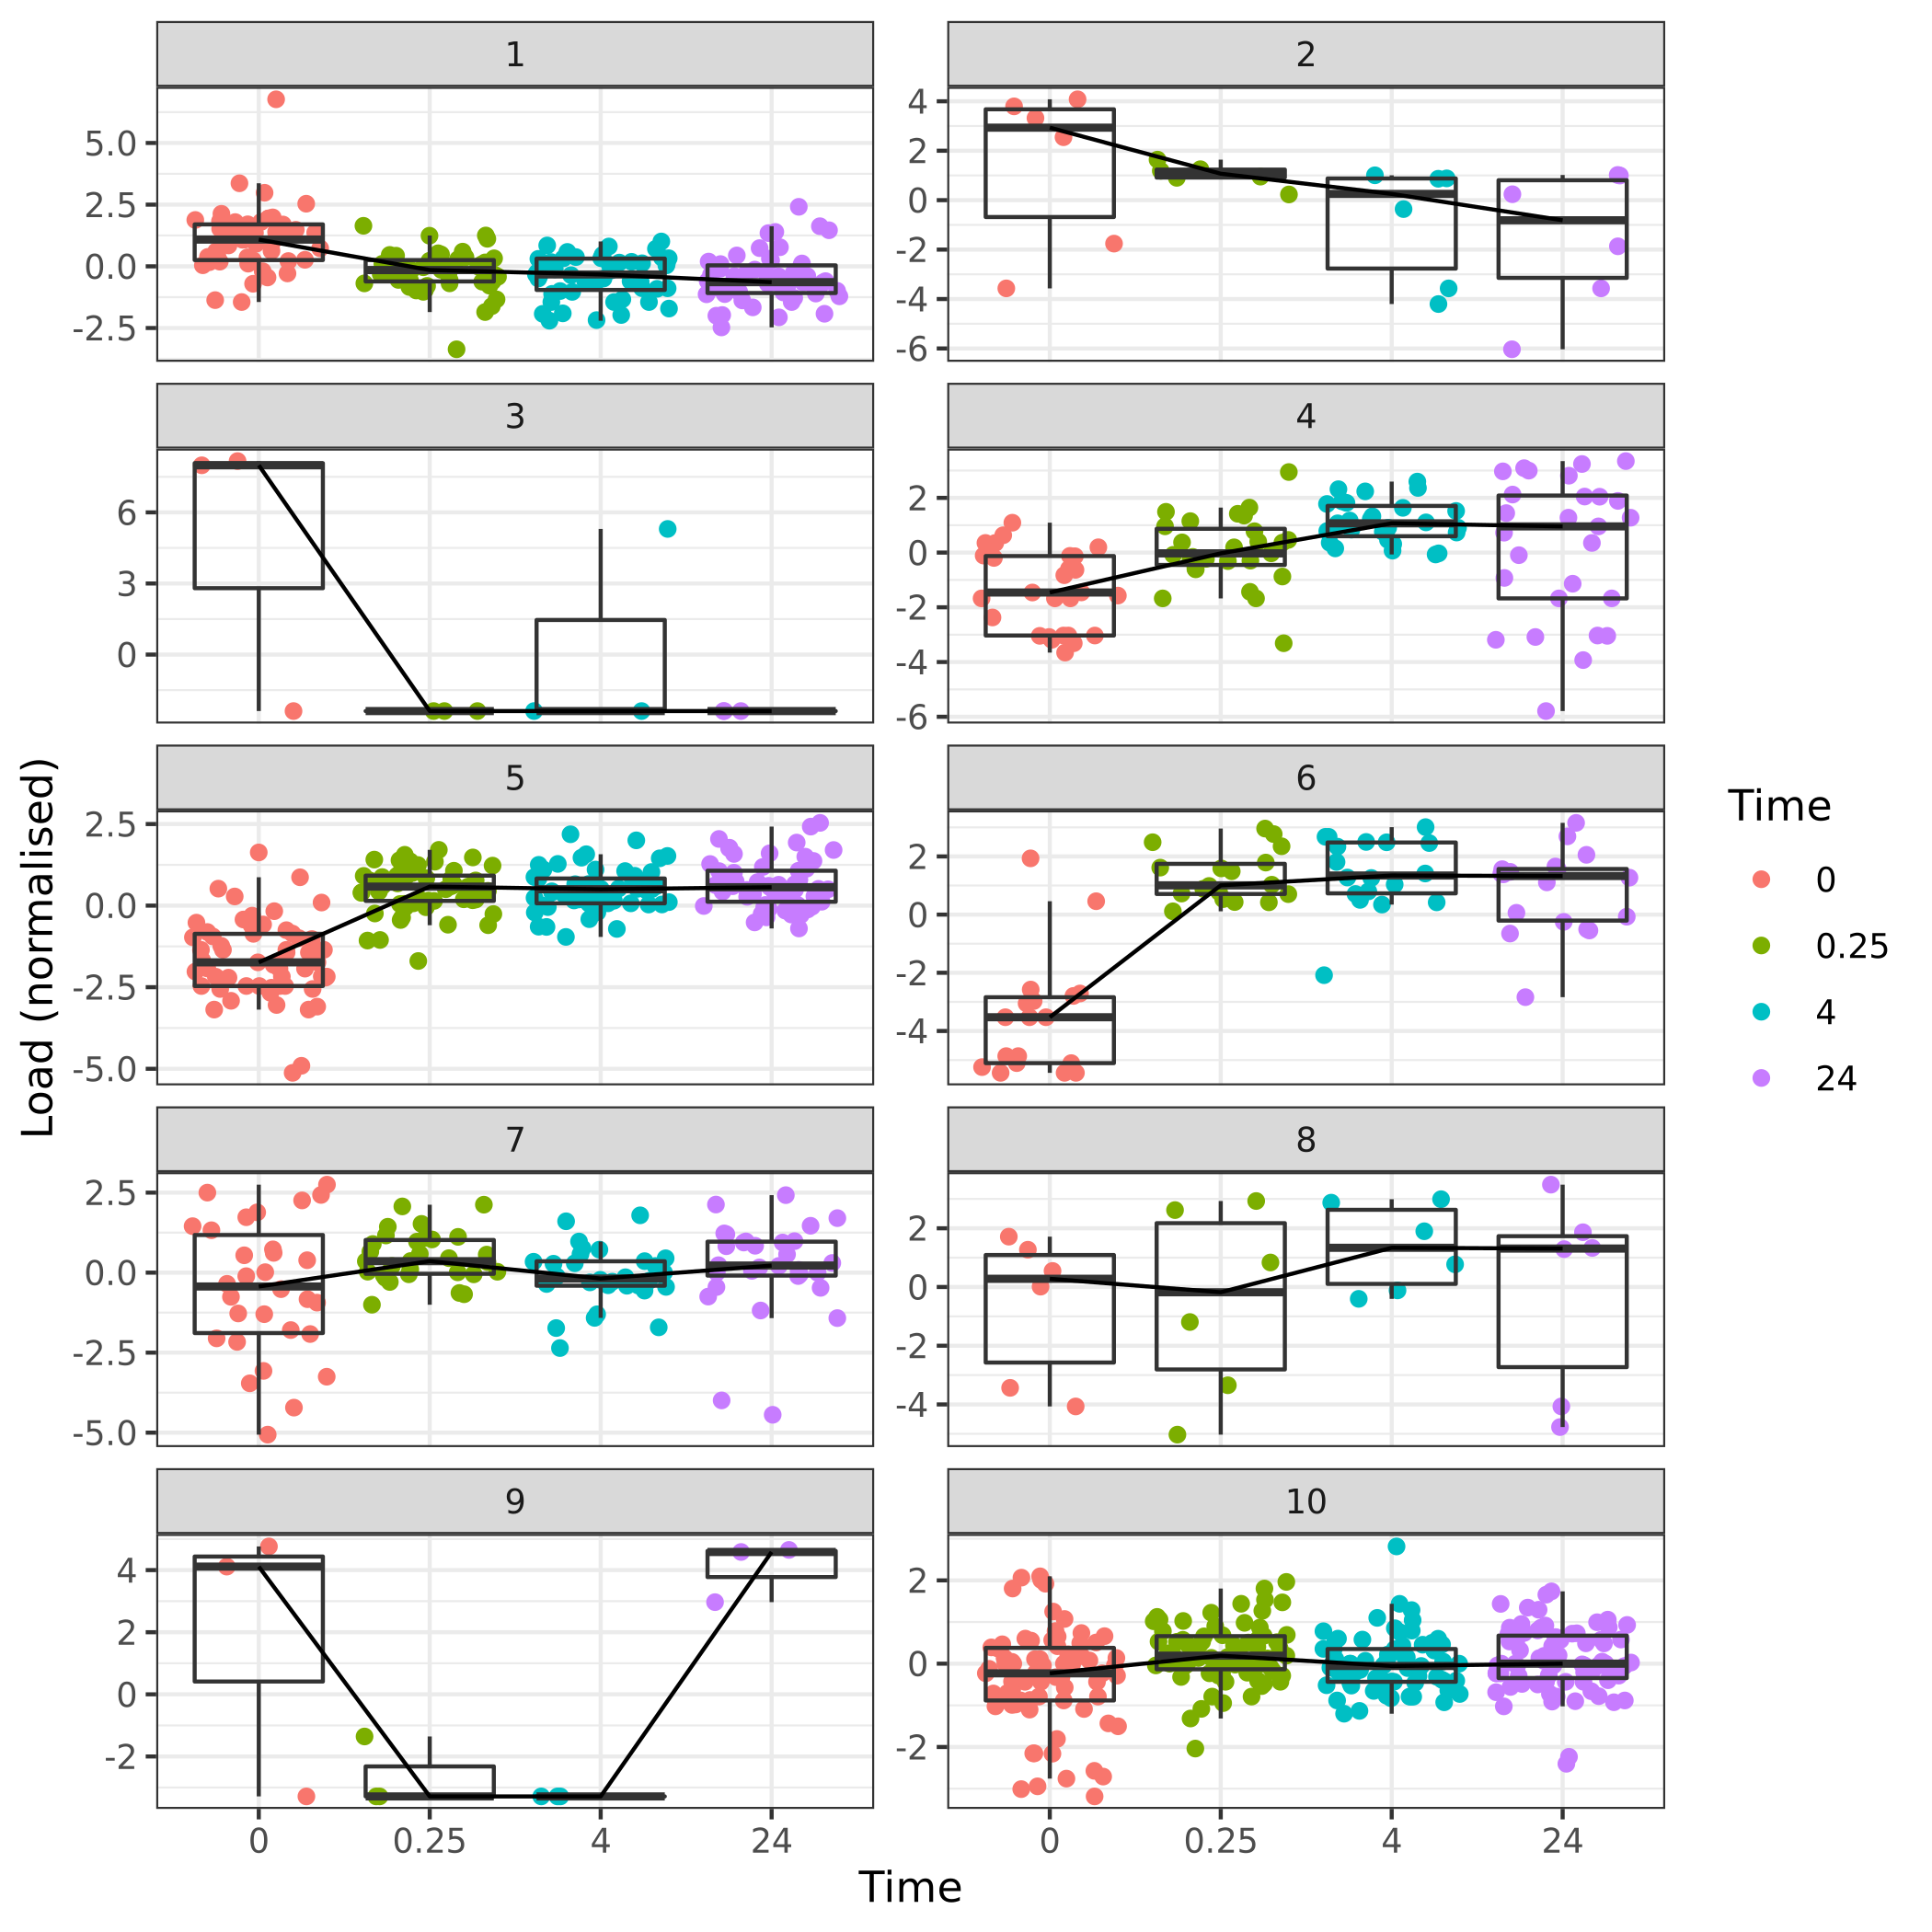
\includegraphics[width=0.6\textwidth]{figure10/PERM/Bodybox.png}
\end{center}
\begin{enumerate}
\item Supplemental Tables
\label{sec:orga0a7bff}
\url{figure10/PERM/Bodybox/}
\end{enumerate}
\subsection{Figure 11: GO analysis (treemaps)}
\label{sec:org6a2089e}

\section{Discussion}
\label{sec:orgd8ac333}
\end{document}
